% Options for packages loaded elsewhere
\PassOptionsToPackage{unicode}{hyperref}
\PassOptionsToPackage{hyphens}{url}
\documentclass[
]{article}
\usepackage{xcolor}
\usepackage{amsmath,amssymb}
\setcounter{secnumdepth}{5}
\usepackage{iftex}
\ifPDFTeX
  \usepackage[T1]{fontenc}
  \usepackage[utf8]{inputenc}
  \usepackage{textcomp} % provide euro and other symbols
\else % if luatex or xetex
  \usepackage{unicode-math} % this also loads fontspec
  \defaultfontfeatures{Scale=MatchLowercase}
  \defaultfontfeatures[\rmfamily]{Ligatures=TeX,Scale=1}
\fi
% \usepackage{lmodern}
\ifPDFTeX\else
  % xetex/luatex font selection
\fi
% Use upquote if available, for straight quotes in verbatim environments
\IfFileExists{upquote.sty}{\usepackage{upquote}}{}
\IfFileExists{microtype.sty}{% use microtype if available
  \usepackage[]{microtype}
  \UseMicrotypeSet[protrusion]{basicmath} % disable protrusion for tt fonts
}{}
\makeatletter
\@ifundefined{KOMAClassName}{% if non-KOMA class
  \IfFileExists{parskip.sty}{%
    \usepackage{parskip}
  }{% else
    \setlength{\parindent}{0pt}
    \setlength{\parskip}{6pt plus 2pt minus 1pt}}
}{% if KOMA class
  \KOMAoptions{parskip=half}}
\makeatother
\usepackage{color}
\usepackage{fancyvrb}
\newcommand{\VerbBar}{|}
\newcommand{\VERB}{\Verb[commandchars=\\\{\}]}
\DefineVerbatimEnvironment{Highlighting}{Verbatim}{commandchars=\\\{\}}
% Add ',fontsize=\small' for more characters per line
\newenvironment{Shaded}{}{}
\newcommand{\AlertTok}[1]{\textcolor[rgb]{1.00,0.00,0.00}{\textbf{#1}}}
\newcommand{\AnnotationTok}[1]{\textcolor[rgb]{0.38,0.63,0.69}{\textbf{\textit{#1}}}}
\newcommand{\AttributeTok}[1]{\textcolor[rgb]{0.49,0.56,0.16}{#1}}
\newcommand{\BaseNTok}[1]{\textcolor[rgb]{0.25,0.63,0.44}{#1}}
\newcommand{\BuiltInTok}[1]{\textcolor[rgb]{0.00,0.50,0.00}{#1}}
\newcommand{\CharTok}[1]{\textcolor[rgb]{0.25,0.44,0.63}{#1}}
\newcommand{\CommentTok}[1]{\textcolor[rgb]{0.38,0.63,0.69}{\textit{#1}}}
\newcommand{\CommentVarTok}[1]{\textcolor[rgb]{0.38,0.63,0.69}{\textbf{\textit{#1}}}}
\newcommand{\ConstantTok}[1]{\textcolor[rgb]{0.53,0.00,0.00}{#1}}
\newcommand{\ControlFlowTok}[1]{\textcolor[rgb]{0.00,0.44,0.13}{\textbf{#1}}}
\newcommand{\DataTypeTok}[1]{\textcolor[rgb]{0.56,0.13,0.00}{#1}}
\newcommand{\DecValTok}[1]{\textcolor[rgb]{0.25,0.63,0.44}{#1}}
\newcommand{\DocumentationTok}[1]{\textcolor[rgb]{0.73,0.13,0.13}{\textit{#1}}}
\newcommand{\ErrorTok}[1]{\textcolor[rgb]{1.00,0.00,0.00}{\textbf{#1}}}
\newcommand{\ExtensionTok}[1]{#1}
\newcommand{\FloatTok}[1]{\textcolor[rgb]{0.25,0.63,0.44}{#1}}
\newcommand{\FunctionTok}[1]{\textcolor[rgb]{0.02,0.16,0.49}{#1}}
\newcommand{\ImportTok}[1]{\textcolor[rgb]{0.00,0.50,0.00}{\textbf{#1}}}
\newcommand{\InformationTok}[1]{\textcolor[rgb]{0.38,0.63,0.69}{\textbf{\textit{#1}}}}
\newcommand{\KeywordTok}[1]{\textcolor[rgb]{0.00,0.44,0.13}{\textbf{#1}}}
\newcommand{\NormalTok}[1]{#1}
\newcommand{\OperatorTok}[1]{\textcolor[rgb]{0.40,0.40,0.40}{#1}}
\newcommand{\OtherTok}[1]{\textcolor[rgb]{0.00,0.44,0.13}{#1}}
\newcommand{\PreprocessorTok}[1]{\textcolor[rgb]{0.74,0.48,0.00}{#1}}
\newcommand{\RegionMarkerTok}[1]{#1}
\newcommand{\SpecialCharTok}[1]{\textcolor[rgb]{0.25,0.44,0.63}{#1}}
\newcommand{\SpecialStringTok}[1]{\textcolor[rgb]{0.73,0.40,0.53}{#1}}
\newcommand{\StringTok}[1]{\textcolor[rgb]{0.25,0.44,0.63}{#1}}
\newcommand{\VariableTok}[1]{\textcolor[rgb]{0.10,0.09,0.49}{#1}}
\newcommand{\VerbatimStringTok}[1]{\textcolor[rgb]{0.25,0.44,0.63}{#1}}
\newcommand{\WarningTok}[1]{\textcolor[rgb]{0.38,0.63,0.69}{\textbf{\textit{#1}}}}
\usepackage{longtable,booktabs,array}
\newcounter{none} % for unnumbered tables
\usepackage{calc} % for calculating minipage widths
% Correct order of tables after \paragraph or \subparagraph
\usepackage{etoolbox}
\makeatletter
\patchcmd\longtable{\par}{\if@noskipsec\mbox{}\fi\par}{}{}
\makeatother
% Allow footnotes in longtable head/foot
\IfFileExists{footnotehyper.sty}{\usepackage{footnotehyper}}{\usepackage{footnote}}
\makesavenoteenv{longtable}
\usepackage{graphicx}
\makeatletter
\newsavebox\pandoc@box
\newcommand*\pandocbounded[1]{% scales image to fit in text height/width
  \sbox\pandoc@box{#1}%
  \Gscale@div\@tempa{\textheight}{\dimexpr\ht\pandoc@box+\dp\pandoc@box\relax}%
  \Gscale@div\@tempb{\linewidth}{\wd\pandoc@box}%
  \ifdim\@tempb\p@<\@tempa\p@\let\@tempa\@tempb\fi% select the smaller of both
  \ifdim\@tempa\p@<\p@\scalebox{\@tempa}{\usebox\pandoc@box}%
  \else\usebox{\pandoc@box}%
  \fi%
}
% Set default figure placement to htbp
\def\fps@figure{htbp}
\makeatother
\setlength{\emergencystretch}{3em} % prevent overfull lines
\providecommand{\tightlist}{%
  \setlength{\itemsep}{0pt}\setlength{\parskip}{0pt}}
\usepackage[]{natbib}
\bibliographystyle{plainnat}
\usepackage{bookmark}
\IfFileExists{xurl.sty}{\usepackage{xurl}}{} % add URL line breaks if available
\urlstyle{same}
\hypersetup{
  colorlinks=true,linkcolor=red,urlcolor=red,citecolor=red,anchorcolor=red,
  pdfcreator={LaTeX via pandoc}}

\author{}
\date{}

\title{Holistic Area Reporting and Living Handbooks\\\normalsize From structured evidence to updated handbook sections}
\author{Area Handbook Author\\\footnotesize{Docxology Template}\\\footnotesize{\texttt{handbook@example.com}}\\\footnotesize{\href{https://orcid.org/0000-0000-0000-0000}{ORCID: 0000-0000-0000-0000}} \\ \footnotesize{2026-03-22}}
\date{2026-03-22}

\usepackage{amsmath}
\usepackage{amssymb}
\usepackage{geometry}
\usepackage{graphicx}
\usepackage{booktabs}
\usepackage{microtype}
\usepackage{hyperref}
\hypersetup{colorlinks=true,allcolors=blue}
\usepackage[capitalise,noabbrev]{cleveref}
\usepackage{natbib}

\begin{document}

\maketitle
\thispagestyle{empty}
\tableofcontents
\newpage


\section{Abstract}\label{abstract}

Holistic area reports aggregate geography, communities, economy,
infrastructure, environment, and governance into a single maintained
narrative. This project treats the \textbf{handbook} as a versioned
artifact: evidence items with themes and weights roll up into
chapter-level coverage scores (with a configurable gap threshold),
unused themes and duplicate corpus ids are detected at load time, and
analysis scripts regenerate figures plus JSON and Markdown rollups from
a committed fixture corpus \citep{bowker2005, template2026}.

The Riverbend Metropolitan Area fixture demonstrates the full path
offline: seventeen evidence rows span eight handbook themes, each row
carrying \texttt{source\_label} and \texttt{reviewed\_at} so reviewers
can see how fresh a claim is without opening side spreadsheets.
Synthesis caps section scores at unity, lists gaps when scores sit
strictly below policy threshold, and emits
\texttt{handbook\_report.json} for dashboards or funder reporting.
Figures show per-section coverage, evidence counts by theme, and
gap-aware coloring so visual review stays aligned with machine-readable
metrics.

The workflow is offline-first, reproducible, and aligned with the
template thin-orchestrator pattern so that prose, code, and outputs stay
traceable across update cycles \citep{edwards2010}. Boundary-style
collaboration---planners, funders, and residents interpreting the same
outline files differently but converging on shared versions---mirrors
how provenance-aware systems stabilize meaning across communities of
practice \citep{gray2005, star1989}. LLM assists are disabled in this
exemplar's \texttt{config.yaml} so CI and local builds remain
deterministic.

\newpage

\section{Introduction}\label{introduction}

Regions, counties, and cross-border metros rarely lack data; they lack
\textbf{shared, maintained synthesis}. Dashboards age, PDFs fork, and
narrative documents drift from underlying sources. A \textbf{living
handbook} addresses this by binding three commitments:

\begin{enumerate}
\def\labelenumi{\arabic{enumi}.}
\tightlist
\item
  \textbf{Structured evidence} --- Each claim carries a theme, source
  label, review date, and explicit weight.
\item
  \textbf{Deterministic rollups} --- Section coverage and gap lists
  derive from the same rules on every build.
\item
  \textbf{Pipeline coupling} --- Figures and tables are regenerated by
  tested scripts before PDF rendering.
\end{enumerate}

Stakeholders include planners, funders, and community liaisons who need
a single entry point that still respects provenance \citep{gray2005}.
Update cadence can follow fiscal quarters, grant milestones, or
incident-driven reviews; the corpus \texttt{version} string records
which snapshot the rendered handbook reflects, while
\texttt{reviewed\_at} on each evidence row signals row-level freshness
inside that snapshot.

The Riverbend Metropolitan Area fixture in
\texttt{data/fixtures/riverbend\_area.yaml} illustrates the pattern
without network calls: it is fictional, exhaustive across declared
themes, and safe for continuous integration. Evidence \texttt{ev-001}
and \texttt{ev-002} anchor the landscape chapter to watershed extent and
post-slide zoning; \texttt{ev-005} through \texttt{ev-008} tie economy
and infrastructure to payroll mix, commute trends, bridge backlog, and
broadband reach. Authoring conventions for this manuscript live in
\url{handbook_syntax.md}.

\textbf{Why YAML first.} The corpus is intentionally flatter than a full
knowledge graph: reviewers can diff pull requests, auditors can grep for
\texttt{source\_label}, and the loader can fail fast on schema
violations \citep{bowker2005}. Bibliographic richness stays in
\texttt{references.bib} for the narrative; the corpus records
\emph{which institutional artifact} backed a row, not a complete
citation object.

\textbf{Roles and boundary objects.} Outline JSON, coverage plots, and
\texttt{handbook\_report.json} function as shared artifacts that
technical staff, policy staff, and external partners interpret
differently while pinning releases to the same file hashes
\citep{star1989}. When a chapter's bar sits left of the gap threshold,
the gap list names a \texttt{section\_id} that is stable in PDF, HTML,
and JSON---reducing translation error between ``the economy chapter
feels thin'' and ``\texttt{06\_economy} is below threshold 0.35.''

\textbf{Scope.} This exemplar does not ingest live APIs, scrape the web,
or resolve DOIs for evidence rows. It shows how a frozen corpus plus
tested Python modules produce reproducible handbook bodies, slides, and
web mirrors under the template pipeline \citep{template2026}.

\newpage

\section{Methods: Corpus model}\label{methods-corpus-model}

The \textbf{area corpus} is a YAML (or JSON) document with:

\begin{itemize}
\tightlist
\item
  \textbf{Identity} --- \texttt{area\_id}, \texttt{area\_label}, and
  semantic \texttt{version}.
\item
  \textbf{Themes} --- Stable identifiers used to route evidence into
  handbook chapters; each theme includes human-readable \texttt{label}
  and \texttt{description} for glossaries and reviewer orientation.
\item
  \textbf{Evidence} --- Atomic statements with \texttt{theme},
  \texttt{weight} in \([0,1]\), \texttt{source\_label}, and
  \texttt{reviewed\_at}.
\end{itemize}

Validation rejects unknown themes, out-of-range or non-finite weights,
blank text fields, \textbf{duplicate} \texttt{themes{[}{]}.id} or
\texttt{evidence{[}{]}.id} values, and missing keys so corrupt files
fail fast at load time. The loader lives in \texttt{src/corpus\_io.py}
and is covered by dedicated tests (including JSON and YAML entry
points).

\textbf{Weights as bounded signals.} Each evidence \texttt{weight} is a
single scalar in \([0,1]\). It is not a probability distribution across
rows; it is a reviewer-assigned strength or credibility hint. During
synthesis, \texttt{section\_coverage\_score()} sums weights for all
evidence whose \texttt{theme} matches a section's \texttt{theme\_ids},
then caps the sum at \(1.0\). That cap prevents stacking many
low-confidence rows into an artificially ``certain'' chapter score.

\textbf{Provenance is intentionally lightweight.} The field
\texttt{source\_label} names the document, export, or system row that
justified the statement---e.g., ``Regional GIS Compendium 2024'' or
``DOT condition database export''---without embedding a full citation
graph in the corpus. Bibliographic detail remains in
\texttt{references.bib} for the manuscript narrative layer.
\texttt{reviewed\_at} uses ISO-8601 dates so freshness checks sort
lexicographically and render cleanly in Markdown tables.

\textbf{Riverbend shape.} The fixture declares eight themes (landscape
through recommendations) and seventeen evidence rows. Every theme
receives at least one row, which yields an empty
\texttt{themes\_without\_evidence} list in metrics---a deliberate
``happy path'' for teaching the pipeline. Sparse corpora in tests
demonstrate the opposite: empty \texttt{themes\_without\_evidence} is
not guaranteed when teams add themes before evidence arrives.

\newpage

\section{Methods: Outline and chapter
routing}\label{methods-outline-and-chapter-routing}

Handbook chapters follow a \textbf{fixed template}
(\texttt{HANDBOOK\_TEMPLATE} in \texttt{src/outline.py}). Each chapter
lists one or more \texttt{theme\_ids}; evidence items whose
\texttt{theme} matches are attached during synthesis.

Ordering is lexicographic by \texttt{section\_id} after discovery in the
manuscript directory; numeric prefixes (\texttt{04\_}, \texttt{05\_},
\ldots) keep print and PDF alignment with the conceptual flow: landscape
through recommendations. The template lists eight sections
(\texttt{04\_landscape} \ldots{} \texttt{11\_recommendations});
manuscript files \texttt{12\_}--\texttt{14\_} extend the bound volume
with maintenance guidance, stakeholder notes, and schema appendix
without altering the core scoring template unless
\texttt{HANDBOOK\_TEMPLATE} is edited in code.

\textbf{One-to-many routing.} A single theme id may feed multiple
sections if the template repeats it, but in this exemplar each
operational theme maps to its namesake chapter. Recommendations-themed
evidence rolls into \texttt{11\_recommendations}; risks-themed evidence
into \texttt{10\_risks}. That keeps reviewer mental models simple: the
YAML \texttt{theme} field is the bucket name reviewers already use in
workshops.

\textbf{Stability for tests and diffs.} The template can later be
parameterized per area (e.g., coastal zones inserting hazard chapters)
while keeping the same synthesis interface. For this exemplar, the
outline is static so tests assert stable section counts, deterministic
score keys, and reproducible \texttt{area\_outline.json}. Any pull
request that changes \texttt{HANDBOOK\_TEMPLATE} should update tests,
fixture expectations, and manuscript headings together.

\textbf{Manuscript discovery.} Rendering combines numbered section
files, optional \texttt{S01\_}--style supplemental markdown, then
glossary and references buckets per
\texttt{infrastructure.rendering.manuscript\_discovery}. Authors should
keep \texttt{section\_id} strings in code, JSON, and filenames aligned
so cross-links and gap reports do not drift.

\newpage

\section{Methods: Synthesis, gaps, and coverage
scores}\label{methods-synthesis-gaps-and-coverage-scores}

\textbf{Synthesis} (\texttt{src/synthesis.py}) maps each handbook
section to the tuple of evidence items whose themes intersect the
section's \texttt{theme\_ids}. The \textbf{coverage score} is computed
by \texttt{section\_coverage\_score()}: the sum of weights for that
section, capped at \(1.0\), so many weak items cannot masquerade as
certainty.

Sections whose score is \textbf{strictly below} the configured gap
threshold (default \texttt{DEFAULT\_GAP\_THRESHOLD\ =\ 0.35}) are listed
in \texttt{gaps}. Callers may pass
\texttt{synthesize(corpus,\ gap\_threshold=…)} when a stricter or looser
policy applies; the chosen value is stored on
\texttt{SynthesisResult.gap\_threshold} and echoed in JSON metrics via
\texttt{build\_metrics\_report()} (\texttt{gap\_threshold},
\texttt{gap\_section\_ids}, \texttt{gap\_count}).

Figure \ref{fig:coverage} shows section-level scores for the Riverbend
fixture. Figure \ref{fig:bytheme} shows how many evidence rows attach to
each theme id in the same fixture. Figure \ref{fig:gapstatus} repeats
the section ordering used in metrics export (sorted ids) and colors bars
by membership in \texttt{gap\_section\_ids}, so readers can see which
chapters would be flagged without rereading JSON.

\begin{figure}
\centering
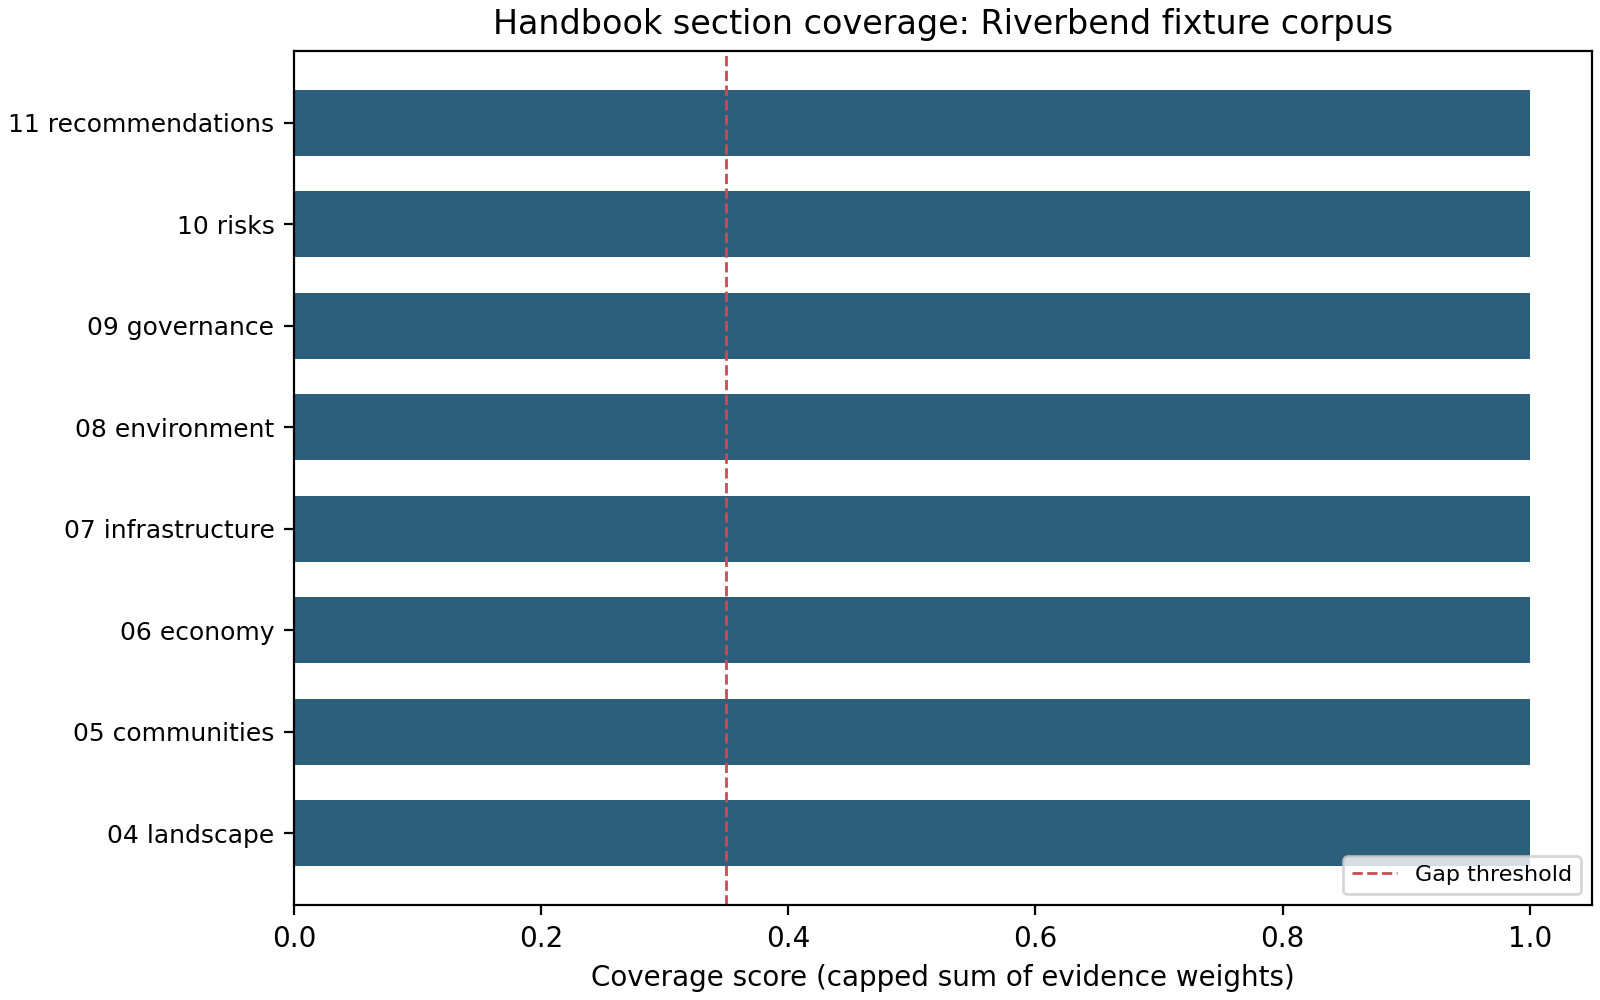
\includegraphics[width=0.85\linewidth,height=\textheight,keepaspectratio,alt={Riverbend fixture (version 2026.1): horizontal coverage score per handbook section (capped sum of matching evidence weights, range 0--1). Red dashed vertical line: current gap threshold from synthesis; sections strictly to the left would be listed in the JSON gaps array.}]{../figures/handbook_evidence_coverage.png}
\caption{Riverbend fixture (version 2026.1): horizontal coverage score
per handbook section (capped sum of matching evidence weights, range
0--1). Red dashed vertical line: current gap threshold from synthesis;
sections strictly to the left would be listed in the JSON gaps
array.}\label{fig:coverage}
\end{figure}

Under the default threshold, the Riverbend exemplar places every outline
section at or above the line (\texttt{gap\_count} is zero in
\texttt{handbook\_report.json}), which is why the executive summary can
describe a ``fully covered'' template run. The chart still documents the
contract: any future corpus revision that drags a section left of the
dashed line will surface automatically in the gap table from
\texttt{build\_gap\_report\_md()} and in pipeline metrics.

\begin{figure}
\centering
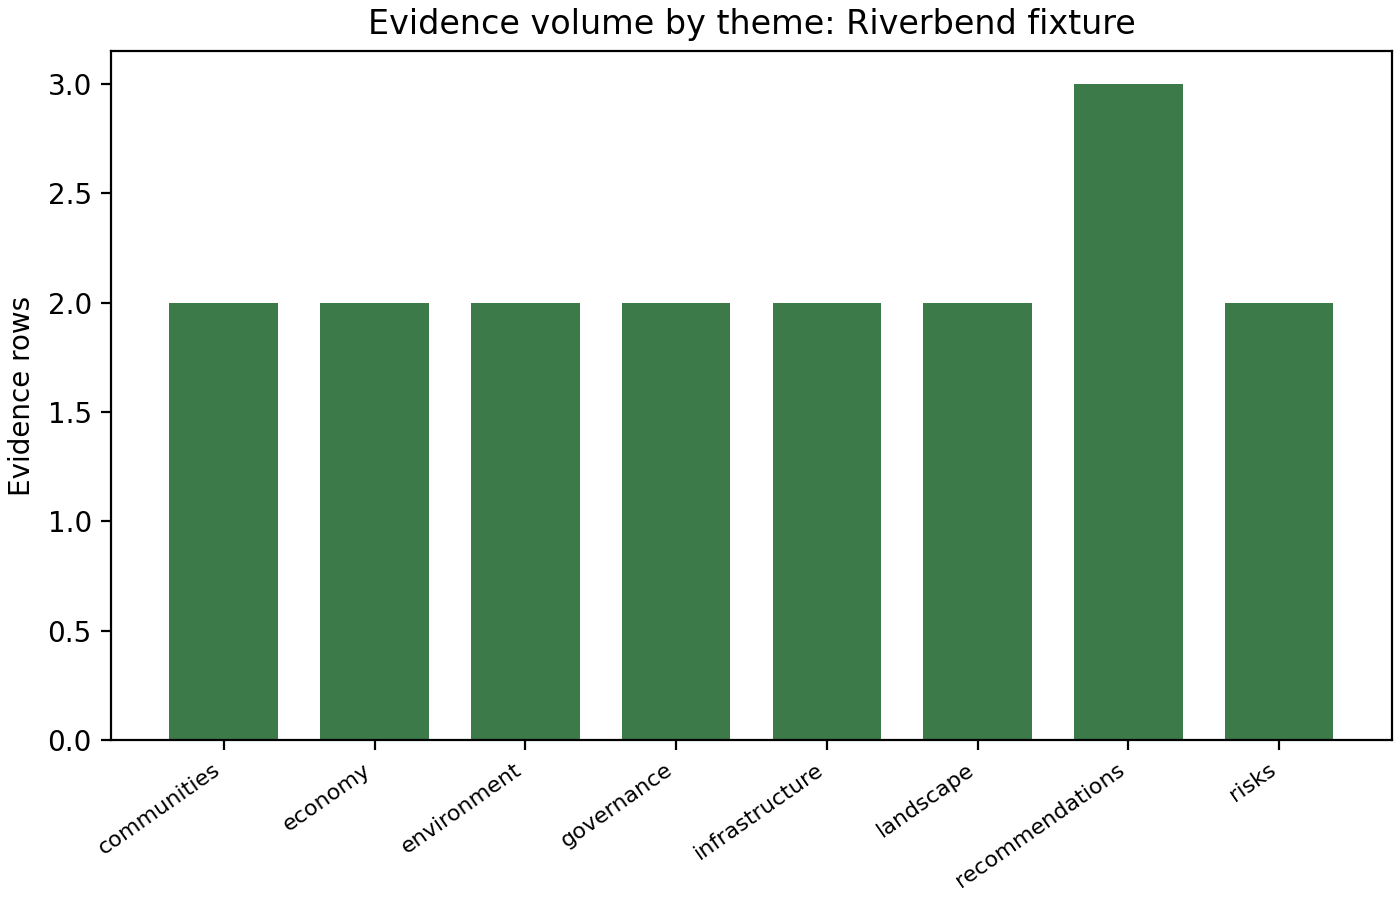
\includegraphics[width=0.8\linewidth,height=\textheight,keepaspectratio,alt={Riverbend fixture: count of evidence rows per theme id after corpus validation (duplicate ids and invalid weights rejected at load). Bar height shows how many statements contribute to each thematic bucket used for section routing.}]{../figures/handbook_evidence_by_theme.png}
\caption{Riverbend fixture: count of evidence rows per theme id after
corpus validation (duplicate ids and invalid weights rejected at load).
Bar height shows how many statements contribute to each thematic bucket
used for section routing.}\label{fig:bytheme}
\end{figure}

The histogram is intentionally simple: it answers whether evidence
volume is balanced across themes or concentrated in a few buckets. For
Riverbend, economy, infrastructure, and recommendations each carry
multiple rows, while every declared theme has at least one row
(\texttt{themes\_without\_evidence} is empty). Editors use this view to
spot missing thematic coverage before rewriting chapter prose.

\begin{figure}
\centering
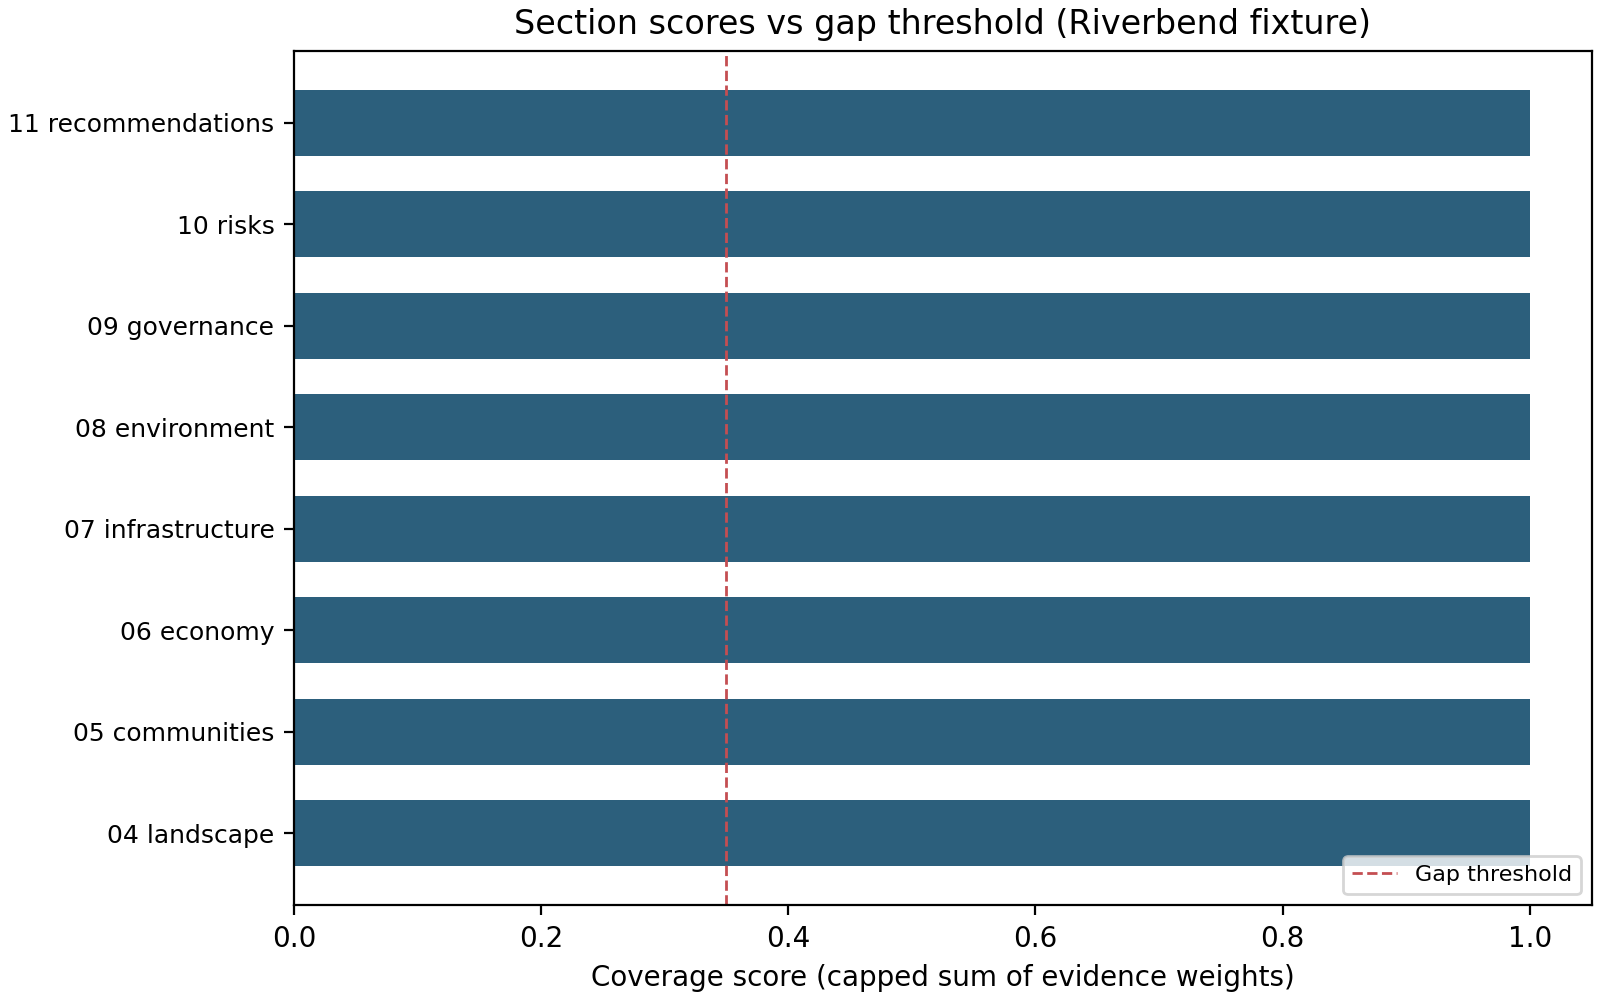
\includegraphics[width=0.85\linewidth,height=\textheight,keepaspectratio,alt={Same scores as the coverage chart, sorted by section id, with bars colored by gap status: coral = section id in gap\_section\_ids (score strictly below threshold); steel blue = at or above threshold. For this fixture under the default threshold, all sections are above the line (empty gap list), illustrating a fully covered outline.}]{../figures/handbook_section_gap_status.png}
\caption{Same scores as the coverage chart, sorted by section id, with
bars colored by gap status: coral = section id in gap\_section\_ids
(score strictly below threshold); steel blue = at or above threshold.
For this fixture under the default threshold, all sections are above the
line (empty gap list), illustrating a fully covered
outline.}\label{fig:gapstatus}
\end{figure}

When \texttt{gap\_section\_ids} is non-empty, coral bars identify
exactly which sections require new evidence or threshold tuning before
publication. The sort order matches \texttt{scores\_by\_section} keys in
JSON, which keeps figure inspection aligned with diff review of
\texttt{handbook\_report.json}.

Markdown bodies for preview or annex publication are assembled in
\texttt{src/handbook\_md.py}: executive bullets, gap table,
evidence-by-theme table, per-section evidence lists, and optional
\texttt{build\_toc\_md()} for outline-only exports.

\newpage

\section{Methods: Quality gates on the corpus
file}\label{methods-quality-gates-on-the-corpus-file}

Before synthesis runs, \texttt{src/corpus\_io.py} rejects files that
would silently corrupt metrics:

\begin{itemize}
\tightlist
\item
  \textbf{Unique ids} --- Duplicate \texttt{themes{[}{]}.id} or
  \texttt{evidence{[}{]}.id} values raise
  \texttt{CorpusValidationError}.
\item
  \textbf{Non-empty text fields} --- Theme \texttt{label} and
  \texttt{description}, evidence \texttt{statement},
  \texttt{source\_label}, and \texttt{reviewed\_at} must be non-blank
  after stripping.
\item
  \textbf{Numeric weights} --- Each \texttt{weight} must parse as a
  finite float in \([0, 1]\) (NaN and infinity are rejected).
\end{itemize}

These checks keep CI deterministic: the same YAML on disk always loads
or always fails with an actionable message. Downstream
\texttt{src/corpus\_stats.py} then reports themes that have
\textbf{zero} evidence rows, which is valid (reserved buckets) but
visible in the executive summary Markdown.

\textbf{Operational implications.} Teams can run the project test suite
locally before pushing corpus edits; failures point to line-level
validation rather than cryptic PDF breaks later. The gates also protect
multi-author editing: two contributors cannot both add \texttt{ev-001}
without merge resolution---the second duplicate id triggers an exception
at load.

\textbf{Cross-field consistency.} Every \texttt{evidence.theme} must
reference an existing \texttt{themes{[}{]}.id}. Typos therefore surface
immediately (``economy'' vs ``economy\_sector'') instead of producing
silent empty matches during synthesis. Combined with the cap on section
scores, these rules keep the handbook honest about what was reviewed and
what was never supplied.

\textbf{Downstream consumers.} \texttt{handbook\_report.json} carries
\texttt{evidence\_count}, \texttt{theme\_count}, \texttt{gap\_count},
and \texttt{themes\_without\_evidence}. Oversight bodies can treat
non-zero \texttt{themes\_without\_evidence} or rising
\texttt{gap\_count} under a fixed threshold as signals to schedule
evidence workshops---not as build failures, but as explicit visibility
\citep{template2026}.

\newpage

\section{Landscape and setting}\label{landscape-and-setting}

Riverbend spans two watersheds feeding a shared estuary; hillside zoning
tightened after repeated slide seasons. These facts anchor
transportation, hazard planning, and conservation priorities.

The corpus ties \textbf{landscape}-themed evidence to this chapter;
synthesis surfaces both strengths (GIS-backed extent data) and places
where only policy narrative exists without quantitative backup.

\textbf{Evidence in the fixture.} Row \texttt{ev-001} (weight 0.9,
Regional GIS Compendium 2024) states the core county spans 420 square
miles with two major watersheds feeding the Riverbend
estuary---establishing geographic scale for every downstream chapter
that references ``the region.'' Row \texttt{ev-002} (weight 0.7, County
zoning bulletin Q3/2025) records hillside development restrictions after
the 2019 slide season, linking land-use law to hazard history. Together
they give handbook authors concrete source labels to echo in prose while
keeping numbers traceable to reviewed rows.

\textbf{Synthesis view.} Landscape evidence is among the
strongest-weighted rows in Riverbend; under the default gap threshold
the landscape section clears the bar with room to spare. If a future
corpus revision removed \texttt{ev-001} or slashed weights, the coverage
chart and \texttt{gap\_section\_ids} would show the regression before
narrative edits masked it.

\textbf{Editorial practice.} When new lidar or watershed models arrive,
add evidence rows rather than overwriting chapter paragraphs alone. Bump
\texttt{version} when those rows materially change scores, and cite the
new \texttt{source\_label} in the handbook text so PDF readers can align
sentences with corpus metadata \citep{edwards2010}.

\newpage

\section{Communities and civic life}\label{communities-and-civic-life}

Unincorporated neighborhoods without chartered councils and
overstretched youth programs illustrate how \textbf{communities}
evidence maps to service gaps. Handbook readers should see both
demographic pressure points and civic infrastructure that still
functions.

Updates to this chapter should add dated evidence rows rather than
rewriting paragraphs ad hoc, preserving auditability.

\textbf{Fixture rows.} \texttt{ev-003} (weight 0.8) reports twelve
unincorporated neighborhoods lack a permanent community council charter,
sourced to an internal civic inventory spreadsheet reviewed 2025-10-18.
\texttt{ev-004} (weight 0.65) notes youth program waitlists exceed
capacity in three east-bank school districts, with the school district
annual report 2025 as provenance. The weight spread reflects slightly
higher confidence in the charter gap count than in the waitlist claim, a
judgment reviewers encode explicitly rather than hiding in prose.

\textbf{Why both rows matter.} Council charters and youth programs are
different failure modes---governance form versus service
throughput---but both sit in the communities theme so synthesis can roll
them into one chapter score. If either row were removed, the section
score would fall, potentially triggering a gap flag under stricter
thresholds.

\textbf{Handbook voice.} Narrative paragraphs can humanize the
spreadsheet facts, but the corpus remains the authority for ``how many
neighborhoods'' and ``which school districts.'' That split mirrors
database provenance practice: store the atomic claim once, reference it
many times \citep{gray2005}.

\textbf{Maintenance.} When a district publishes a new annual report, add
a superseding row or bump \texttt{reviewed\_at} on a revised statement;
avoid silent edits that leave old dates on new numbers.

\newpage

\section{Economy and livelihoods}\label{economy-and-livelihoods}

Sector concentration (healthcare and logistics) and lengthening commutes
describe a labor market that is employed yet stressed for time.
\textbf{Economy} evidence items capture payroll composition and
travel-cost signals.

Economic narratives in the handbook should cite the same source labels
as the corpus so PDF and data exports do not diverge.

\textbf{Evidence detail.} \texttt{ev-005} (weight 0.85, State labor
market review) states healthcare and logistics account for 34\% of
payroll employment region-wide---a single scalar summarizing sector
concentration. \texttt{ev-006} (weight 0.55, ACS five-year comparison)
records median commute time rose six minutes between 2018 and 2024
despite flat population, signaling time poverty even when headcounts
hold steady. The lower weight on \texttt{ev-006} invites future
corroboration from employer surveys or mode-share data without
discarding the commute signal today.

\textbf{Reading the charts.} In Figure \ref{fig:bytheme}, economy shares
the bar chart with other themes; Riverbend carries two economy rows,
matching the two statements above. Coverage charts show how those rows
combine with the template's \texttt{theme\_ids} for \texttt{06\_economy}
to produce a bounded section score.

\textbf{Policy links.} Concentration and commute duration interact with
infrastructure and environment chapters: bridge delays and heat exposure
can compound commute stress. Cross-chapter reading is intentional; the
risks chapter (\texttt{10\_risks}) names systemic couplings explicitly.

\textbf{Data hygiene.} When labor market reviews update NAICS rollups or
ACS releases new vintages, add rows or deprecate old ones in the corpus
rather than patching PDFs only \citep{bowker2005}.

\newpage

\section{Infrastructure and
connectivity}\label{infrastructure-and-connectivity}

Bridge maintenance backlogs and uneven broadband coverage are classic
\textbf{infrastructure} themes. The fixture encodes both physical asset
risk and digital divide geography.

Handbook maintenance teams can prioritize bond packages or grant
applications using gap flags when coverage scores fall below policy
thresholds.

\textbf{Evidence rows.} \texttt{ev-007} (weight 0.9, DOT condition
database export) states deferred bridge maintenance spans 47 structures
flagged as priority repair---high confidence because asset registries
are auditable. \texttt{ev-008} (weight 0.75, Broadband map consortium)
reports fiber-to-premises coverage reaches 78\% of households with rural
gaps along the northern ridge. Together they pair heavy civil liability
with last-mile equity, a common pairing in regional handbooks.

\textbf{Synthesis and finance.} Strong weights on both rows help the
infrastructure section score stay robust under default thresholds. If
bond scoring workflows consume \texttt{handbook\_report.json}, teams can
watch \texttt{scores\_by\_section} for \texttt{07\_infrastructure}
alongside raw evidence counts to see whether narrative urgency matches
quantitative backing.

\textbf{Digital divide nuance.} The broadband row is explicitly
geographic (``northern ridge''), which handbook prose should preserve
rather than generalizing to ``rural areas'' without naming the ridge
feature, unless new evidence broadens the claim.

\textbf{Operations.} When DOT exports a new quarterly extract, version
the corpus and add or update rows so \texttt{reviewed\_at} reflects the
extract date \citep{template2026}.

\newpage

\section{Environment and stewardship}\label{environment-and-stewardship}

Wildland-urban interface expansion and improved sewer overflow
performance sit in tension: growth pressure versus capital investment
wins. \textbf{Environment} evidence should be reviewed after major
projects or regulatory cycles.

Linking environmental claims to dated review metadata avoids stale
hazard language after remediation.

\textbf{Rows in Riverbend.} \texttt{ev-009} (weight 0.7, Remote sensing
memo 2025) documents wildland-urban interface acres grew 11\% since the
last land-cover assessment---framing exposure growth independent of any
single fire event. \texttt{ev-010} (weight 0.6, Water authority annual
compliance letter) notes combined sewer overflows dropped after the
north interceptor project went online, tying infrastructure capital to
ambient water-quality outcomes.

\textbf{Tension as a feature.} The handbook presents both statements in
one chapter so readers cannot pretend growth and compliance are
unrelated. Synthesis still produces a single score; authors interpret
trade-offs in prose while the corpus preserves the underlying claims
with weights reflecting reviewer confidence.

\textbf{Review cadence.} Land-cover assessments arrive on multi-year
cycles; compliance letters annually or on permit schedules.
\texttt{reviewed\_at} should jump when those documents refresh;
otherwise dashboards overstate freshness \citep{edwards2010}.

\textbf{Cross-links.} Heat and hydrology threads continue in
\texttt{10\_risks} and \texttt{07\_infrastructure}; environment evidence
here grounds those discussions in stewardship and regulatory
performance.

\newpage

\section{Governance and services}\label{governance-and-services}

Overlapping special districts and aging emergency-plan synchronization
are \textbf{governance} concerns that span jurisdictions. The handbook
makes fragmentation visible without pretending a single author owns all
fixes.

Cross-reference the risks chapter when governance gaps amplify single
points of failure (e.g., shared river crossings).

\textbf{Fixture evidence.} \texttt{ev-011} (weight 0.8, Interlocal
services audit) reports nine special districts overlap tax boundaries in
the central corridor, complicating service accounting. \texttt{ev-012}
(weight 0.45, State readiness checklist) states emergency operations
plans were last synchronized across counties in 2021---a lower-weight
row flagging stale coordination that may need tabletop exercises to
refresh.

\textbf{Interpreting weights.} The emergency-plan row carries the lowest
weight among Riverbend governance items, signaling uncertainty about
whether 2021 remains accurate or whether partial updates occurred
without a full sync. Handbook authors should describe that nuance;
reviewers can raise the weight after a new statewide drill report enters
the corpus.

\textbf{Service accounting.} Overlapping districts often confuse
residents during tax mailings; the handbook can cite \texttt{ev-011}
when explaining why service maps disagree across PDFs from different
agencies \citep{star1989}.

\textbf{Risks coupling.} Freight dependence on a single river crossing
(\texttt{ev-014} in the risks chapter) becomes more alarming when
governance synchronization lags (\texttt{ev-012}). Narrative
cross-references help readers connect institutional drift to physical
vulnerability.

\newpage

\section{Cross-cutting risks}\label{cross-cutting-risks}

Heat trends and freight dependence on one river crossing compound one
another. \textbf{Risks} evidence is intentionally cross-domain so
readers see systemic coupling, not siloed hazards.

Scenario planning exercises can attach new evidence rows after each
tabletop drill, bumping the corpus version when the handbook is
regenerated.

\textbf{Evidence.} \texttt{ev-013} (weight 0.85, NOAA station history)
states heat-wave days above 95°F have doubled in the last two decades at
the airport station---climate exposure anchored to a specific observing
site. \texttt{ev-014} (weight 0.7, Freight model technical appendix)
notes a single river crossing carries 62\% of east-west freight truck
trips, concentrating economic and emergency risk on one structure.

\textbf{Compounding.} Either hazard alone warrants attention; together
they stress cooling centers, detour capacity, and redundant corridors.
The handbook's risks chapter is where such interactions belong, even
when thematic evidence also appears under environment or infrastructure.

\textbf{Figures.} Section coverage plots (Figure \ref{fig:coverage})
include \texttt{10\_risks}; gap status coloring (Figure
\ref{fig:gapstatus}) applies the same threshold logic. Under Riverbend
defaults all sections pass, but a sparse risks portfolio would show
coral bars here first.

\textbf{After-action reviews.} Each drill or incident should yield dated
rows: new \texttt{reviewed\_at}, possibly new \texttt{source\_label}
strings pointing to after-action PDFs. That habit keeps the living
handbook aligned with operational learning \citep{template2026}.

\newpage

\section{Recommendations}\label{recommendations}

Prioritized actions in the fixture include data-sharing agreements,
bridge maintenance bonds, and resilience hub pilots.
\textbf{Recommendations} carry the highest weights where consensus
already exists in source documents.

The handbook is not a substitute for democratic deliberation; it is a
structured rollup of what evidence-backed proposals are on the table at
version print time.

\textbf{Rows.} \texttt{ev-015} (weight 0.9, Regional planning task force
draft) calls for a recurring interagency data sharing agreement for
transit and land use permits. \texttt{ev-016} (weight 0.88, DOT capital
program white paper) proposes funding a five-year bridge maintenance
bond aligned to the priority repair list---directly echoing
infrastructure evidence about deferred repairs. \texttt{ev-017} (weight
0.72, Heat equity working group) pilots neighborhood resilience hubs in
districts with longest cooling-center travel times, linking
recommendations to risks and communities chapters without duplicating
their evidence ids.

\textbf{Weight ordering.} The data-sharing row tops the weight list
among recommendations, signaling strongest reviewer confidence or
institutional buy-in in this fictional exercise. Weights are not votes;
they guide synthesis caps and gap detection, not automatic budget
allocation.

\textbf{Narrative boundaries.} Recommendations prose should clarify that
inclusion in the corpus does not imply adoption by any elected body
\citep{bowker2005}. The corpus records that a proposal was documented
and reviewed on a date, not that it passed a council vote.

\textbf{Versioning.} Task-force drafts evolve quickly; when PDFs
supersede one another, update \texttt{source\_label} strings or add
successor rows so readers know which draft the handbook referenced.

\newpage

\section{Handbook maintenance}\label{handbook-maintenance}

A living handbook requires \textbf{three operational habits}:

\begin{enumerate}
\def\labelenumi{\arabic{enumi}.}
\tightlist
\item
  \textbf{Version the corpus} when evidence changes materially.
\item
  \textbf{Run analysis scripts} before rendering so figures and JSON
  match the corpus.
\item
  \textbf{Archive PDFs} with the corpus version in metadata or filename.
\end{enumerate}

The template pipeline encodes steps 2--3; teams adopt step 1 through
governance. Optional LLM assists are disabled in \texttt{config.yaml}
for this exemplar to keep builds deterministic.

\textbf{Pull-request discipline.} Treat \texttt{riverbend\_area.yaml}
(or production corpora) like code: require review, run
\texttt{uv\ run\ pytest\ projects/area\_handbook/tests/}, and attach
\texttt{handbook\_report.json} diffs when scores move. Figure
regeneration via \texttt{scripts/02\_generate\_handbook\_figure.py}
updates PNGs and \texttt{figure\_registry.json}, keeping validation
green in \texttt{04\_validate\_output.py}.

\textbf{Release artifacts.} Ship three bundles together: the corpus file
at a tagged version, \texttt{handbook\_report.json}, and the combined
PDF (or HTML). Consumers can then verify that narrative, metrics, and
data describe the same snapshot \citep{gray2005}.

\textbf{Threshold policy.} Changing \texttt{DEFAULT\_GAP\_THRESHOLD} in
code alters which sections gap without any prose edit. Document
threshold policy in steering minutes and prefer explicit
\texttt{synthesize(...,\ gap\_threshold=...)} in custom scripts if
regional policy diverges from repository defaults.

\textbf{Supplemental sections.} Files such as \texttt{S01\_*.md} and
\texttt{S02\_*.md} follow manuscript discovery ordering; add them when
limitations or worked examples grow too long for the main chapter flow.

\textbf{Slides and web.} The same markdown feeds Beamer slides and
static web mirrors; maintenance includes checking relative figure paths
after directory moves and confirming browser loads for
\texttt{output/web/index.html} after each major template upgrade
\citep{template2026}.

\newpage

\section{Stakeholders and use cases}\label{stakeholders-and-use-cases}

\textbf{Regional planners} use the handbook as a single narrative spine
across departments; the corpus gives them a checklist of which chapters
still lack reviewed evidence. Shared artifacts such as the outline JSON
and coverage figures act as \textbf{boundary objects} in the sense of
\citet{star1989}: different groups attach different meanings while
aligning on the same file versions.

\textbf{Funders and oversight bodies} can require a corpus version
string and the \texttt{handbook\_report.json} metrics block as
deliverables, without mandating a particular writing style in the prose
chapters. \texttt{coverage\_ratio}, \texttt{gap\_count}, and
\texttt{total\_evidence\_weight} summarize whether the outline is backed
at the threshold encoded in the build---useful for pass/fail gates on
grants.

\textbf{Community liaisons} benefit when gap sections name
\texttt{section\_id} codes that map back to outline rows---those ids are
stable across PDF, HTML, and JSON exports. When a chapter is thin,
liaisons can translate \texttt{06\_economy} into plain language without
losing traceability to the same machine-readable key funders see.

\textbf{Tooling maintainers} extend \texttt{HANDBOOK\_TEMPLATE} in
\texttt{src/outline.py} when new policy domains appear (e.g., housing,
broadband equity), then add matching themes to the YAML schema and
manuscript files in the same pull request. Skipping any leg of that
triangle yields empty scores or orphan markdown files.

\textbf{Emergency managers and public works directors} may never edit
YAML; they consume PDFs and slides. For them, figures such as Figure
\ref{fig:bytheme} communicate whether thematic buckets are balanced,
while Figure \ref{fig:gapstatus} shows whether any section failed the
gap policy on the last build.

\textbf{Researchers studying provenance} can treat the corpus as a
bounded case of lightweight metadata practice: enough structure for
automation, not so much that community partners cannot contribute rows
\citep{gray2005}.

The Riverbend fixture is intentionally \textbf{fictional} so public
repos can ship a full worked example without redacting real resident
data.

\newpage

\section{Appendix: YAML corpus schema (normative
summary)}\label{appendix-yaml-corpus-schema-normative-summary}

{\def\LTcaptype{none} % do not increment counter
\begin{longtable}[]{@{}
  >{\raggedright\arraybackslash}p{(\linewidth - 4\tabcolsep) * \real{0.2188}}
  >{\raggedright\arraybackslash}p{(\linewidth - 4\tabcolsep) * \real{0.3438}}
  >{\raggedright\arraybackslash}p{(\linewidth - 4\tabcolsep) * \real{0.4375}}@{}}
\toprule\noalign{}
\begin{minipage}[b]{\linewidth}\raggedright
Field
\end{minipage} & \begin{minipage}[b]{\linewidth}\raggedright
Location
\end{minipage} & \begin{minipage}[b]{\linewidth}\raggedright
Constraint
\end{minipage} \\
\midrule\noalign{}
\endhead
\bottomrule\noalign{}
\endlastfoot
\texttt{area\_id} & root & Non-empty string \\
\texttt{area\_label} & root & Non-empty string \\
\texttt{version} & root & Non-empty string (semantic or calendar
versioning recommended) \\
\texttt{themes} & root & Non-empty list of objects with \texttt{id},
\texttt{label}, \texttt{description} \\
\texttt{evidence} & root & List (may be empty) of objects with
\texttt{id}, \texttt{statement}, \texttt{theme}, \texttt{weight},
\texttt{source\_label}, \texttt{reviewed\_at} \\
\end{longtable}
}

Each \texttt{evidence.theme} must equal some \texttt{themes{[}{]}.id}.
Weights are unitless credibility or strength signals capped per row at
\(1.0\); section scores cap the sum per chapter at \(1.0\) in
\texttt{src/synthesis.py}.

\textbf{Example evidence object (Riverbend).}

\begin{Shaded}
\begin{Highlighting}[]
\KeywordTok{{-}}\AttributeTok{ }\FunctionTok{id}\KeywordTok{:}\AttributeTok{ ev{-}007}
\AttributeTok{  }\FunctionTok{statement}\KeywordTok{:}\AttributeTok{ Deferred bridge maintenance now spans 47 structures flagged as priority repair.}
\AttributeTok{  }\FunctionTok{theme}\KeywordTok{:}\AttributeTok{ infrastructure}
\AttributeTok{  }\FunctionTok{weight}\KeywordTok{:}\AttributeTok{ }\FloatTok{0.9}
\AttributeTok{  }\FunctionTok{source\_label}\KeywordTok{:}\AttributeTok{ DOT condition database export}
\AttributeTok{  }\FunctionTok{reviewed\_at}\KeywordTok{:}\AttributeTok{ }\StringTok{"2025{-}11{-}28"}
\end{Highlighting}
\end{Shaded}

\textbf{Example theme object.}

\begin{Shaded}
\begin{Highlighting}[]
\KeywordTok{{-}}\AttributeTok{ }\FunctionTok{id}\KeywordTok{:}\AttributeTok{ infrastructure}
\AttributeTok{  }\FunctionTok{label}\KeywordTok{:}\AttributeTok{ Infrastructure}
\AttributeTok{  }\FunctionTok{description}\KeywordTok{:}\AttributeTok{ Transport, utilities, broadband, and maintenance backlogs.}
\end{Highlighting}
\end{Shaded}

Machine-readable outline and metrics after a build:

\begin{itemize}
\tightlist
\item
  \texttt{projects/area\_handbook/output/data/area\_outline.json}
\item
  \texttt{projects/area\_handbook/output/data/handbook\_report.json}
\item
  \texttt{projects/area\_handbook/output/data/handbook\_toc.md}
\end{itemize}

The combined human-readable rollup lives in \texttt{handbook\_body.md}
in the same directory.

\textbf{Figures and registry.} Running
\texttt{scripts/02\_generate\_handbook\_figure.py} writes PNGs under
\texttt{projects/area\_handbook/../figures/} and updates
\texttt{figure\_registry.json} for validation. Manuscript labels
\texttt{fig:coverage}, \texttt{fig:bytheme}, and \texttt{fig:gapstatus}
must stay aligned with that script.

\textbf{Empty evidence list.} An empty \texttt{evidence} array still
instantiates all template sections with score zero; metrics report
\texttt{gap\_count} equal to section count. This edge case is tested to
prevent divide-by-zero surprises in coverage ratios.

\textbf{JSON interchange.} \texttt{load\_corpus\_from\_dict} accepts
Python dicts shaped like parsed JSON for tests and API adapters; the
same constraints as YAML apply \citep{template2026}.

\newpage

\section{Supplement: Limitations and
assumptions}\label{supplement-limitations-and-assumptions}

This exemplar prioritizes \textbf{reproducibility and teachability} over
geographic realism. Riverbend is fictional; weights and source labels
illustrate schema use, not empirical findings about any jurisdiction.

\textbf{No live data.} The pipeline does not call HTTP APIs, scrape
documents, or perform NLP on attachments. Every number in the handbook
narrative traces to a hand-authored YAML row or to derived metrics
computed from those rows.

\textbf{Weights are subjective.} Reviewers assign \texttt{weight} in
\([0,1]\) without a universal rubric. Cross-team calibration is a
governance task outside this repository; the code assumes weights are
already consensus values.

\textbf{Single corpus per build.} The scripts load one fixture path
(\texttt{data/fixtures/riverbend\_area.yaml} in production use of this
demo). Merging multiple corpora or federating regions would require new
modules and tests, not configuration toggles alone.

\textbf{Outline static in code.} \texttt{HANDBOOK\_TEMPLATE} is Python
source, not a per-area YAML file. Customizing chapters without editing
code is possible only within the existing section files and themes;
adding a ninth scored section demands code and test updates.

\textbf{Citation depth.} \texttt{source\_label} is a short string, not a
BibTeX key. Formal citations belong in manuscript markdown using
\texttt{references.bib}; the corpus stays lean \citep{bowker2005}.

\textbf{Threshold semantics.} ``Gap'' means strictly below threshold,
not ``close.'' Sections barely above the line still pass; policy teams
may want stricter thresholds or secondary rules implemented in future
metrics fields.

\newpage

\section{Supplement: Worked example --- reading Riverbend end to
end}\label{supplement-worked-example-reading-riverbend-end-to-end}

This note walks a reviewer from fixture file to rendered artifacts
without running commands, highlighting how ids line up across layers.

\textbf{1. Load and validate.} \texttt{src/corpus\_io.load\_corpus}
reads \texttt{riverbend\_area.yaml}, checks ids, weights, and theme
membership, and builds an \texttt{AreaCorpus} object. Failure modes
include duplicate \texttt{ev-001} or a \texttt{weight} of \texttt{nan}.

\textbf{2. Outline.} \texttt{build\_handbook\_outline} returns
\texttt{HANDBOOK\_TEMPLATE}: eight sections from \texttt{04\_landscape}
through \texttt{11\_recommendations}, each with \texttt{theme\_ids} that
pick up matching evidence.

\textbf{3. Synthesis.} \texttt{synthesize} attaches evidence to
sections, sums weights with a cap of \(1.0\), compares each score to
\texttt{DEFAULT\_GAP\_THRESHOLD} (0.35), and fills \texttt{gaps} with
ids strictly below threshold. Riverbend under defaults yields an empty
gap tuple because every section clears the bar.

\textbf{4. Metrics JSON.} \texttt{build\_metrics\_report} flattens
scores, gap lists, theme histograms, and descriptive stats. A CI job can
assert \texttt{evidence\_count\ ==\ 17} and
\texttt{themes\_without\_evidence\ ==\ {[}{]}} for this fixture.

\textbf{5. Markdown bodies.} \texttt{build\_full\_handbook\_body} emits
section headings, evidence lists, and tables suitable for annex
publication; \texttt{handbook\_toc.md} mirrors outline depth.

\textbf{6. Figures.} \texttt{02\_generate\_handbook\_figure.py} plots
scores, theme counts, and gap-colored bars, then registers
\texttt{fig:coverage}, \texttt{fig:bytheme}, and \texttt{fig:gapstatus}
in \texttt{figure\_registry.json} so \texttt{validate\_figure\_registry}
passes during output validation.

\textbf{7. Manuscript.} Numbered markdown sections plus this
supplemental file combine through manuscript discovery; Pandoc assigns
figure numbers from attributes \texttt{\{\#fig:...\}} while preserving
\texttt{\textbackslash{}ref\{...\}} in PDF.

\textbf{Traceability spot check.} If prose cites ``47 priority
bridges,'' the reviewer should find \texttt{ev-007} with that statement
and DOT export provenance. If not, the narrative drifted from the corpus
\citep{gray2005}.

\newpage

\section{Manuscript syntax (area
handbook)}\label{manuscript-syntax-area-handbook}

\subsection{Citations}\label{citations}

Use Pandoc bracket cites with keys from \texttt{references.bib}:

\begin{Shaded}
\begin{Highlighting}[]
\NormalTok{See }\CommentTok{[}\OtherTok{@bowker2005; @template2026}\CommentTok{]}\NormalTok{ for context.}
\end{Highlighting}
\end{Shaded}

\subsection{Figures}\label{figures}

Analysis writes PNGs under \texttt{../figures/}. Reference from
markdown:

\begin{Shaded}
\begin{Highlighting}[]
\AlertTok{![Coverage by section](../figures/handbook\_evidence\_coverage.png)}\NormalTok{\{\#fig:coverage width=85\%\}}

\AlertTok{![Evidence counts by theme](../figures/handbook\_evidence\_by\_theme.png)}\NormalTok{\{\#fig:bytheme width=80\%\}}

\AlertTok{![Gap status by section](../figures/handbook\_section\_gap\_status.png)}\NormalTok{\{\#fig:gapstatus width=85\%\}}
\end{Highlighting}
\end{Shaded}

Run \texttt{scripts/02\_generate\_handbook\_figure.py} via the pipeline
before rendering (also refreshes
\texttt{../figures/figure\_registry.json}).

\subsection{Section files}\label{section-files}

Numbered prefixes \texttt{01\_}--\texttt{14\_} and
\texttt{03a}--\texttt{03d} sort in the main manuscript group. This file
lives in the \textbf{other} discovery bucket (name does not start with a
digit or \texttt{S01\_} pattern) and is ordered lexicographically among
other non-main files---keep the filename stable so build logs stay
predictable.



\bibliography{references}
\end{document}
